\documentclass{article}
\usepackage{graphicx} % Required for inserting images
\usepackage{xcolor}
\usepackage{fancyvrb}
\usepackage{hyperref} % Add this in the preamble
\hypersetup{
    colorlinks=true, % Set to true to color links instead of red boxes
    linkcolor=blue,   % Color of internal links (sections, TOC)
    filecolor=magenta,
    urlcolor=cyan,
    citecolor=blue
}
\usepackage{authblk}

\title{Remote Patient Monitoring\\Assurance Case Development}
\author[1]{Vasilis Athanasiou}
\author[2]{Rance DeLong}
\author[1]{Andreas Menychtas}
\affil[1]{BioAssist}
\affil[2]{The Open Group}
}
\date{January 2026}

\begin{document}

\maketitle
\tableofcontents
\clearpage
\section{Introduction}
We discuss the evolution of the Remote Patient Monitoring (RPM) assurance case as the O-ETB tool developers interact with the RPM assurance case authoring team.
This is a living document to provide a channel for substantive communication about the development and a place to share material that is candidate for inclusion in a future publication.

Because there was not a pre-existing catalog of argument patterns for MedSecurance generally, or for RPM specifically, we encouraged the RPM AC authors to work top-down to create an outline of the assurance case for their use case.
This activity inspired the creation of the Assurance Case Outline (ACO) subsystem in O-ETB.
In this ``living memo'' we follow the evolution of the RPM assurance case outline ("RPM ACO").

%\section{Early ACO versions and tooling efforts}
We started by suggesting that the RPM AC authors begin their assurance case construction top-down by starting with the high level goals and refining downward toward evidence.
As they proceeded with this and shared their early versions we saw a need to put forth some conventions in writing such outlines and an opportunity to provide some machanical support.
The conventions generally followed the GSN Standard to the extent that it was compatible with the implemented O-ETB processor.
The support opportunity was seen as lightweight checking of the conventions and formatting the assurance case outline in several useful ways.
Initially this was seen as a preliminary step toward defining applicable assurance case argument patterns in the Argument Pattern Languate (APL) of the O-ETB Assurance tool to use in transliterating the assurance case outline being developed into instantiations of the defined argument patterns.

The definition of conventions enabled the mechanical support opportunity to quickly develop into a syntax checker and translator from ACO to APL providing a pathway to a complete pipeline to rendered assurance cases in the Certification Assurance Package area for exported assurance cases in txt and html (with graphics) formats.

\clearpage
\section{Applying Kelly’s Six-Step Method to the RPM Case}
\label{sec:kelly}

\subsection{Kelly’s Six-Step Method for GSN construction}
For reference we reiterate Tim Kelly's Six-Step Method (pictured in Figure~\ref{fig:6-step}):
\label{sec:kelly-6-step}
\begin{enumerate}
    \item Identify goals to be supported: Define the main, high-level safety goal (e.g., "The system is safe to operate").
    \item Define basis on which goals stated: Identify the context, assumptions, and constraints under which these goals are made.
    \item Identify strategy to support goals: Choose the strategy or argument approach that explains how the goal will be supported (e.g., decomposing by system component, functional area, or lifecycle phase).
    \item Define basis on which strategy stated: Justify the strategy chosen in Step 3, ensuring it is valid and clearly defined.
    \item Elaborate argument to next level: Break down the goals into lower-level sub-goals (decomposition) based on the strategy.
    \item Identify grounded premises: Connect the lowest-level sub-goals to actual evidence (solutions, data, tests, analysis) that supports them. 
\end{enumerate}
\begin{figure}[h]
    \centering
    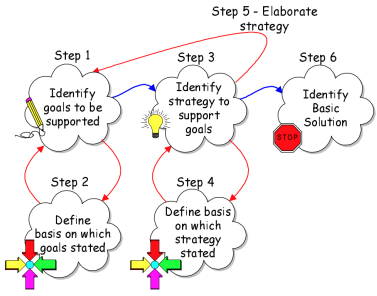
\includegraphics[width=0.5\linewidth]{6-step.png}
    \caption{Kelly's 6-Step Method}
    \label{fig:6-step}
\end{figure}

In the initial development of an assurance case it is natural to identify the top-level goals and to define subgoal structure under those.
The decomposition continues until the kind of evidence needed to support the goal structure can be identified.
This activity is primarily of the Steps 1, 3, 5 and 6 variety.
At this stage there are typically unstated assumptions and implicit context, which should be made explicit by
the continuing refinement of the case so that it can be examined and tested to provide coherence, precision and rigour. Steps 2 and 4 drive this refinement.


\subsection{The Role of Kelly’s ``Define the Basis'' Steps 2 and 4}
\label{sec:kelly-basis}

Kelly’s six-step method for constructing assurance arguments explicitly distinguishes between claims and strategies on the one hand, and the \emph{basis} on which those claims and strategies are stated on the other. In both the original formulation and the later Hawkins--Kelly refinement, this distinction plays a critical role in ensuring that arguments are not only structured, but also meaningful and robust.

\paragraph{Step 2: Define the basis on which the claim is stated.}
This step concerns the \emph{meaning} of the claim: the scope, definitions, assumptions, and interpretations that must be fixed in order for the claim to be unambiguous. Without an explicit basis, claims may be interpreted differently by different readers, or may drift in meaning as the assurance case evolves.

\paragraph{Step 4: Define the basis on which the strategy is stated.}
This step concerns the \emph{reasoning premises} underlying the chosen argument strategy: why this particular way of arguing is appropriate, and under what assumptions it is expected to be sufficient. Step~4 makes explicit the premises that connect evidence to claims, and therefore plays a key role in managing inductive gaps and confidence in the argument.

In practice, these ``basis'' steps serve as the semantic anchor for the entire argument structure. When they are weak or implicit, refinement tends to proceed by embedding explanation into evidence nodes or by overloading goals with unstated assumptions. This leads to bloated nodes and large abstraction gaps that become increasingly difficult to manage as the case grows.

\subsubsection{Application to the RPM assurance case}

In the BIO assurance case, much of the initial development has proceeded top--down, with high--level goals elaborated before the underlying vocabulary and scope were fully stabilized. This is a natural and productive way to begin, but it places additional importance on later attention to Kelly’s Steps~2 and~4.

Several of the refinement transformations illustrated in this document---particularly T1 (Evidence node slimming), T2 (Intermediate goal insertion), and T4 (Evidence category grounding)---implicitly depend on a clear and shared basis. For example:

\begin{itemize}
  \item Determining whether an evidence item can directly discharge a goal depends on a precise understanding of what the goal actually asserts.
  \item Grounding an evidence category requires agreement on what counts as an artifact of a given type, and in what context it is valid.
  \item Distinguishing identification from compliance (as in the regulatory example) requires explicit scoping assumptions.
\end{itemize}

By making basis material explicit, these dependencies are addressed directly rather than being left implicit and compensated for elsewhere in the argument.

\subsubsection{Relationship to Ontology and Vocabulary Discipline in MedSecurance}

Kelly’s basis steps can be viewed as the assurance--case analogue of establishing a shared and stable vocabulary. They do not require a fully developed formal ontology from the outset, but they do benefit from deliberate attention to terminology, scope, and classification.

In the context of MedSecurance, a project--level ontology is maintained to provide a common vocabulary across tools, methods, and assurance artifacts. While this ontology is defined at the project level, it may admit conservative extensions for particular use cases where additional distinctions are required.

From an assurance--case perspective, Kelly’s ``define the basis'' steps imply a corresponding discipline: the concepts and terms used in claims, strategies, and evidence descriptions should either already be defined in the project ontology, or be treated as candidates for inclusion in an appropriate extension. Where such ontologies already exist, they can be referenced or reused; where they are still evolving, the assurance case itself can help surface which distinctions and definitions are most critical to stabilize.

Importantly, the goal at this stage is not to require assurance--case authors to perform ontology engineering, but to ensure that the meanings on which arguments rely are explicit, reviewable, and consistent across the project. When an assurance case surfaces new or refined concepts that are critical to interpretation, this provides useful feedback to the project ontology rather than a divergence from it, and reduces the need for compensatory explanation elsewhere in the assurance case.


\clearpage
\section{RPM Assurance Case}

\subsection{RPM Assurance Case Outline (ACO)}

Picking up the story at version 5, the RPM AC authors were encouraged to elaborate on the evidence in version 5 and to tie it to MedSecurance methods and tools. This resulted in version 6.
Since version 6 otherwise maintains much of the structure and content of version 5 we will not comment further on version 5 here.

We consider version 6 of the RPM assurance case, the version we are working with at the time of this memo.
Sometimes we will show the .aco input and in other cases, as noted, we will show the txt export of the instantiated assurance case at the end of the pipeline:
$${ACO \rightarrow APL \rightarrow REPOSITORY \rightarrow CAP}$$

Also a graphical representation of the AC can be exported as HTML in the CAP.

Note that the text in the examples presented here have in many cases been \emph{paraphrased} from the actual txt export of the RPM assurance case \emph{solely for compactness} of presentation.
The paraphrase may not faithfully convey the full import and information content of the original text, but has been deemed adequate for the specific issue being illustrated.
In cases where the paraphrasing interferes with the issue to be illustrated, the full original text of the .aco or .txt will be used and so noted. The ``Kelly Steps'' referenced in this section were explained in Section~\ref{sec:kelly}.

\subsection{Exemplars for refinement transformations}
We choose a few evidence nodes for further development with the hope of establishing an example of the kind of further refinement that should be applied to other evidence nodes currently represented in the assurance case.

\subsubsection{Evidence nodes in Data-in-Transit goal G112}
We show in the following extract from the txt export of the assurance case two example evidence nodes, E1121 and E1122, in the context consisting of the path of ancestor nodes up to the root node (G0 bioassistAssuredUse).
\begin{Verbatim}[commandchars=\\\{\}]
G0  bioassistAssuredUse
  "BioAssist provides acceptable protection of patient health and multimedia data"

  G1  confidentiality
    "PHR and multimedia data are protected against unauthorized disclosure"

    G11  clientCloudTransitConfidential
      "Data in transit between clients and BioAssist cloud is confidential"

      G112  secureExternalServiceTransit
        "Data in transit to/from external cloud data sources is encrypted"

        G1121  secureChannelsToExternalSources
          "External API calls use secure channels and authenticated endpoints"

          \color{blue}E1121  apiGatewaySecurityConfiguration
            \color{blue}"Architecture model lists external interfaces; comms reports show
            \color{blue}TLS with authenticated endpoints"

        G1122  noUnprotectedProtocolsForPHRData
          "No sensitive PHR data is sent over unprotected or legacy protocols"

          \color{blue}E1122  networkTrafficAndPenetrationTestResults
            \color{blue}"TVRA model covers PHR data flows; threat analysis shows no
            \color{blue}cleartext-transmission threats"
\end{Verbatim}
This gives a good sense of the context of the evidence nodes under scrutiny.

\subsubsection{Evidence node E1122}
First we will focus on the second evidence node E1122 and the goal it is intended to discharge:

\begin{Verbatim}[commandchars=\\\{\}]
    G1122  noUnprotectedProtocolsForPHRData
      "No sensitive PHR data is sent over unprotected or legacy protocols"
    
      \color{blue}E1122  networkTrafficAndPenetrationTestResults
        \color{blue}"TVRA model covers PHR data flows; threat analysis shows no
        \color{blue}cleartext transmission threats"
\end{Verbatim}
At present the pre-paraphrased E1122 is very \emph{fat}, it is doing too much work: it names an analysis, summarizes its outcome and implicitly asserts adequacy. To close the gap between the parent goal and an evidence artifact we introduce an intermediate goal that can be directly discharged by the evidence artifact.
\begin{Verbatim}[commandchars=\\\{\}]
    G1122a  externalDataFlowThreatsAnalyzed
      "Threats to PHR data confidentiality during external data flows
      have been systematically identified and assessed"
\end{Verbatim}
Now the structure becomes:
\begin{Verbatim}[commandchars=\\\{\}]
    G1122  noUnprotectedProtocolsForPHRData
      G1122a  externalDataFlowThreatsAnalyzed
        \color{blue}E1122  …
\end{Verbatim}
Next we \emph{slim-down} the evidence node E1122, factoring out argumentation, so that it names the artifact rather than arguing from it.
\begin{Verbatim}[commandchars=\\\{\}]
    \color{blue}E1122  tvraExternalDataFlowAnalysis
      "Threat and Vulnerability Risk Analysis (TVRA) report for BioAssist
      external PHR data flows"
\end{Verbatim}
Now it provides no conclusions or justifications.
It just introduces an artifact that can be inspected.
Now that context and justification have been factored-out, they can be added
as supporting nodes under G1122a so that each node does \emph{one} job:
\begin{Verbatim}[commandchars=\\\{\}]
G112  secureExternalServiceTransit
  "Data in transit to/from external cloud data sources is encrypted"

  G1122  noUnprotectedProtocolsForPHRData
    "No sensitive PHR data is sent over unprotected or legacy protocols"
      
    \color{blue}G1122a  externalDataFlowThreatsAnalyzed
      \color{blue}"Threats to PHR data confidentiality during external data
      \color{blue}flows have been systematically identified and assessed"
            
      \color{blue}C1122a  tvraMethodContext
        \color{blue}"TVRA is used in MedSecurance to analyze confidentiality
        \color{blue}threats and vulnerabilities associated with system data flows"
                
      \color{blue}J1122a  tvraAdequacyRationale
        \color{blue}"The TVRA process systematically enumerates threats and
        \color{blue}evaluates mitigations for identified data flows,
        \color{blue}providing a sound basis for confidentiality assessment"

      \color{blue}E1122  tvraExternalDataFlowAnalysis
        \color{blue}"Threat and Vulnerability Risk Analysis (TVRA) report for
        \color{blue}BioAssist external PHR data flows"
\end{Verbatim}
In the transformed assurance case fragment, G112 and G1122 claims are preserved.
The additional intermediate goal clarifies reasoning.
Context and justification are identified and \emph{appropriately placed}.
The evidence node is \emph{thinner} and cleaner:
The new evidence node refers specifically to an \emph{evidence category} (risk/vulnerability analysis), to a \emph{context} (PHR data flows), to a \emph{tool} (TVRA tool), and to a particular artifact form (TVRA report).
The overall case fragment is now easier to read and extend.

\subsubsection{Evidence node E1121}

The following txt export extract shows the E1121 evidence node in context. It emphasizes system modeling to establish claim strength.
\clearpage
\begin{Verbatim}[commandchars=\\\{\}]
  G112  secureExternalServiceTransit
    "Data in transit to/from external cloud data sources is encrypted"

    G1121  secureChannelsToExternalSources
      "External API calls use secure channels and authenticated endpoints"

      \color{blue}E1121  apiGatewaySecurityConfiguration
        \color{blue}"Architecture model lists external interfaces; comms reports show
        \color{blue}TLS with authenticated endpoints"
\end{Verbatim}

Evaluating this evidence node against the Kelly ``Steps,'' the greatest weakness is in Step 4, ``basis of strategy,'' which is completely missing. Also for Step 2, the ``basis of claim'' is implicit rather than explicit. For Step 3, the ``strategy'' is implicit but clear, but the Step 5 ``strategy elaboration'' is minimal.
Step 1 ``claim'' is clear and appropriately scoped, and Step 6 is concrete with identified tools.

We now proceed to address these weaknesses.
Implicitly, the strategy is \emph{to demonstrate that all external API calls use secure channels by showing that every modelled external interface has a communications risk-assessment report recording encrypted, authenticated channels.} It is a design-time, model-based sufficiency strategy. This is a valid and often used approach but its premises should be explicit apart from the evidence item. We suggest that the needed premises are:
\begin{itemize}
    \item Coverage -- ``The architecture/integration model identifies each external cloud data source interface used for ingestion.''
    \item Correspondence -- ``Communications risk-assessment reports correspond to the modelled interfaces.''
    \item Semantic sufficiency -- ``Encrypted channel with authenticated endpoints'' is sufficient to establish ``secure channels'' for the purposes of this claim.
    \item Temporal stability -- ``The reports are representative of operational behavior, not merely design intent.''
\end{itemize}
These statements are not evidence \emph{per se} but rather reasoning assumptions (per Step 4).
To remedy the deficiency we will introduce a justification node to provide our strategy basis.
\begin{Verbatim}[commandchars=\\\{\}]
goal G1121_1 (secureChannelsToExternalSources)
  All outbound and inbound API calls to external sources use
  secure channels (e.g., TLS) and authenticated endpoints.

  strategy S1121_1 (argueSecureTransitByModelAndPerInterfaceReports)
    Argument by
    (i) enumerating all external interfaces in the
    architecture/integration model, and
    (ii) showing that each enumerated interface has a
    communications risk-assessment report recording
    encryption and authenticated endpoints.

    context C1121_1_modelScope
      The architecture/integration model is the authoritative
      design-time enumeration of BioAssist external cloud data
      source interfaces used for ingestion.

    justification J1121_1_strategyBasis
      Basis/premises for this strategy:
        (a) coverage: all external API calls to external sources
        correspond to modelled interfaces;
        (b) correspondence: each modelled interface has an
        associated communications risk-assessment report;
        (c) semantic sufficiency: “encrypted channel with
        authenticated endpoints” suffices to establish “secure
        channel” for this claim;
        (d) stability/fidelity: report conclusions reflect
        the configured/deployed interface behavior for the
        assessed baseline.

    goal G1121a_1 (modelEnumeratesExternalInterfaces)
      All relevant external interfaces are enumerated
      in the model.

      evidence E1121a_1 (architectureIntegrationModelExport)
        Artifact: Export of the BioAssist architecture/integration
        model enumerating external cloud data source interfaces
        used for ingestion.
        Tool: IoMT Model-Based Engineering Tool.
    
    goal G1121b_1 (eachEnumeratedInterfaceIsEncrypted)
      Each enumerated interface is recorded as
      encrypted+authenticated in the risk reports.
            
      evidence E1121b_1 (commsRiskAssessmentReportBundle)
        Artifact: Communications risk-assessment report
        set for external interfaces enumerated in G1121a_1.
        Tool: IoMT Communications Recommendation Tool.
\end{Verbatim}

The transformation adds and modifies some nodes:
\begin{itemize}
    \item The new strategy node carries the form of the reasoning (``enumerate interfaces'' + ``show property per interface'').
    \item The new justification node carries the premises for sufficiency of the strategy.
    \item The new context node identifies the scope of information supplied by the model.
    \item Two intermediate goals that can be directly discharged by the evidence.
    \item The evidence node has been split into two slim ones, each relating to one concrete artifact and the tool that produces it. Each discharges the respective goal.
\end{itemize}

We separate the tools used to produce the evidence item (Step 6) from why that evidence is considered sufficient (Step 4).
This gives a reviewer an opportunity to accept the reasoning apart from considering the proffered evidence item(s).
Thus E1121 does not require new evidence to be more defensible, it only requires explicit premises for reasoning that results in the two intermediate goals that can be directly discharged by the evidence and separating the evidence into the two distinct pieces.


\subsubsection{Evidence node E511 in applicable regulations goal G51 }
The following txt export extract shows the E511 evidence node in context of its path from the root. It illustrates the intended role of this branch: establishing the compliance scope and providing a basis for subsequent compliance argumentation.

\begin{Verbatim}[commandchars=\\\{\}]
G0  bioassistAssuredUse
  "BioAssist provides acceptable protection of patient health and
  multimedia data"

  G5  regulatoryCompliance
    "BioAssist addresses applicable regulatory and standards requirements"

    G51  applicableRegulationsIdentified
      "Relevant regulations and standards for BioAssist are identified"

      G511  regulatoryMappingDocument
        "A regulatory mapping document lists each applicable law or standard
        and the relevant requirements"

        E511  reviewedComplianceMatrix
          "Ontology query enumerates applicable obligations; a matrix maps
          obligations to BioAssist controls and is reviewed/signed off"
\end{Verbatim}

In its original form, E511 is \emph{fat} in the same sense as E1121 and E1122: it simultaneously names a tool, summarizes multiple artifacts, and implicitly asserts sufficiency (coverage/completeness) and trustworthiness (review/sign-off). Those are distinct argumentative roles. When they are collapsed into one evidence node, key premises remain implicit and the branch becomes difficult to refine or audit.

Applying the Kelly 6-step discipline makes the missing structure clear:

\begin{itemize}
\item Kelly Step 2 (define the basis on which the claim is stated): clarify what counts as \emph{applicable} regulation/standard and what it means to \emph{map} an obligation to a control, including the intended scope (system boundary, jurisdictions of deployment, and data types).
\item Kelly Step 4 (define the basis on which the strategy is stated): justify why ontology-based retrieval plus a compliance mapping matrix plus review/sign-off is expected to be sufficient, complete, and trustworthy for discharging the goal.
\end{itemize}

The transformation therefore separates (a) the \emph{meaning} of the claim (Step 2) from (b) the \emph{premises that justify the chosen reasoning approach} (Step 4), and decomposes the branch so that each evidence node names a concrete artifact that can directly discharge a narrowly stated goal.

First, we introduce an explicit Step 2 context node under G511 to normalize the meaning of ``applicable'' and of ``mapping'':

\begin{verbatim}
Context C511_claimBasis:
  Applicability is defined with respect to the RPM system scope,
  jurisdictions of deployment, and the handling of personal health and
  multimedia data; mapping an obligation to a control means identifying
  one or more RPM controls that collectively address the intent of
  that obligation.
\end{verbatim}

Next, we introduce an explicit strategy node under G511 that captures the intended argument form, and we add Step 4 basis material (context/justification) that makes strategy sufficiency premises explicit. The strategy is: (i) enumerate applicable regulations and obligations from the MedSecurance project knowledge base, and (ii) map each obligation to corresponding RPM controls in a reviewed compliance mapping matrix. The Step 4 basis nodes capture the implicit premises that would otherwise remain buried inside the evidence narrative: coverage (that the retrieved set is complete for the declared scope), correctness (that the knowledge base reflects authoritative interpretations), correspondence (that obligations can be mapped to controls), sufficiency (that such mappings are an adequate basis for downstream compliance argumentation), and assurance (that review/sign-off provides confidence in the mapping’s correctness).

Finally, we decompose the original E511 into two dischargeable subgoals, each supported by a slim evidence node:

\begin{itemize}
\item G511a discharges the \emph{enumeration} aspect via a recorded ontology query result (tool output).
\item G511b discharges the \emph{mapping} aspect via a compliance mapping matrix artifact that records mappings and sign-off.
\end{itemize}

The transformed assurance case fragment (as reflected in bio\_v6d.aco) is:

\begin{Verbatim}[commandchars=\\\{\}]
Goal G511 regulatoryMappingDocument:
  A regulatory mapping document exists that enumerates applicable
  regulations and maps their obligations to RPM controls.

  Context C511_claimBasis:
    Applicability is defined with respect to the RPM system
    scope, jurisdictions of deployment, and the handling of personal
    health and multimedia data; mapping an obligation to a control
    means identifying one or more RPM controls that collectively
    address the intent of that obligation.

  Strategy S511 argueRegulatoryCoverageByOntologyAndMatrix:
    Argue regulatory identification and obligation coverage by
    (i) deriving the set of applicable regulations and obligations
    from the project knowledge base and
    (ii) mapping each obligation to corresponding RPM controls
    in a reviewed compliance matrix.

    Context C511_scopeAndAuthority:
      The MedSecurance project knowledge base is the authoritative
      source for determining applicability of regulations and standards
      for personal health and multimedia data handling within the
      defined RPM system scope.

    Justification J511_strategyBasis:
      Basis for this strategy:
      (a) completeness: the ontology query retrieves all regulations
      and obligations applicable to the RPM data types and
      operational context;
      (b) correctness: the ontology encodes current and authoritative
      regulatory interpretations;
      (c) correspondence: each retrieved obligation can be meaningfully
      mapped to one or more RPM controls;
      (d) sufficiency: documented mappings provide an adequate basis
      for downstream compliance argumentation;
      (e) assurance: review and sign-off by compliance/legal personnel
      provides confidence in the correctness of the mapping.

    Goal G511a applicableRegulationsEnumerated:
      All regulations and standards applicable to RPM are
      enumerated with their relevant obligations.

      Evidence E511a ontologyQueryResult:
        Artifact: Recorded ontology query result enumerating
        applicable regulations, standards, and obligations for
        RPM data handling.
        Tool: Ontology-based Knowledge Repository.

    Goal G511b obligationsMappedToControls:
      Each applicable obligation is mapped to one or more RPM
      controls.

      Evidence E511b complianceMappingMatrix:
        Artifact: Compliance mapping matrix mapping regulatory
        obligations to RPM controls, reviewed and signed off
        by compliance/legal personnel.
\end{Verbatim}

This transformation has the same net effect as in the E1121/E1122 examples: it reduces the gap between goal and evidence by introducing directly-dischargeable intermediate goals, and it relocates sufficiency and trustworthiness premises from the evidence node into explicit Step 2/4 basis nodes where they can be reviewed, challenged, and maintained. It also improves extensibility: for example, if applicability must later be supplemented by jurisdiction-specific legal interpretation, this can be added as an explicit extension to the Step 2 basis without rewriting the strategy.


\clearpage
\section{Transformation operations}

In the course of making the previously described refinements to the RPM assurance case, the transformations performed are named and generalized in this section.
It is expected that the collection of transformations will grow with continuing work.

The author is currently relied upon to recognize the applicability of the transformations and to manually apply them.
However, we are currently in the process of automating both of these steps in the form of suggestions to the author and automated application of the suggested transformations upon the author's selection among alternatives and approval.

\subsection{T0 -- Partition the assurance case}
As a new assurance case being developed gets larger, or an existing assurance case is growing due to continuing development, the case may be wide but shallow because top-level goals have been elaborated but not thoroughly refined.
If the assurance case is large and monolithic is should be partitioned into sub-cases along the top-level goals.
If the assurance case is very large, even if partitioned at the top level, further partitioning at lower levels will facilitate further refinement because the author can effectively "zoom in" on parts of the assurance case without being overwhelmed by the size of the entire case.

Partitioning is a principle that should be applied by the author in an ongoing manner throughout the development and refinement of the assurance case.
Presently, partitioning can be effected using transformation T6, the first of the transformations to be automated, and it should be repeated as necessary to keep the assurance case manageable.

\emph{Intent:} Improve continuing development and reviewability by reducing overwhelm and by making the case easier to navigate and focus on cohesive parts separately, without changing the substance of any claim or evidence.

\subsection{T1 -- Evidence node slimming}
If the leap from a goal node to an evidence node spans a large abstraction gap then much of the explanation of the gap may be placed into the evidence node, making it bloated and requiring it to do multiple jobs.
By factoring out context and justification the burden on the evidence node can be reduced.
These aspects can be allocated to nodes of the appropriate type, appropriately placed (see T3).

\emph{Intent:} Ensure each evidence node identifies an inspectable artifact, while explanatory and adequacy reasoning is relocated to appropriately typed nodes.

\subsection{T2 -- Intermediate goal insertion}
Introduce an intermediate goal that can be directly discharged by the evidence.
This transformation is useful when a case is being developed top-down or outside-in, which leads to broad conceptual, abstraction or detail gaps between goal nodes and evidence nodes written to support them.
The goal supported by an evidence item should be \emph{directly discharged} by that item. This transformation may need to be applied repeatedly along with T1 and T3 after T4.

\emph{Intent:} Make implicit reasoning steps explicit by introducing a goal that can be directly discharged by a specific evidential artifact, thereby reducing abstraction gaps.

\subsection{T3 -- Context and justification placement}
Context and justification material should be placed in the corresponding node type and appropriately placed attached to a goal or strategy node to which it is most closely aligned.

\emph{Intent:} Separate meaning (definitions, scope, assumptions) from reasoning sufficiency, improving both traceability and alignment with Kelly Steps~2 and~4.

\subsection{T4 -- Evidence category grounding}
The evidence node should identify:
\begin{itemize}
    \item evidence category
    \item artifact form
    \item the artifact (value) that makes the support relation valid
    \item the artifact producing tool
    \item execution context -- what context information is required by the tool
\end{itemize}
It should not go beyond this or it will be overburdened with information that belongs elsewhere.
Ideally these items should be based on an established taxonomy, or at least one that is being deliberately developed in parallel with the assurance case.

\emph{Intent:} Stabilize how evidence categories are interpreted by mapping them to concrete artifact forms and production contexts, improving reviewer comprehension and consistency.

\subsection{T5 -- Basis Definition and Normalization}
\label{sec:t5}

As assurance cases grow in size and detail, ambiguity in terminology, scope, and interpretation becomes a significant impediment to further refinement.
This ambiguity often manifests as excessive explanation embedded in goal, strategy, or evidence nodes, or as subtle inconsistencies in how key terms are used across different parts of the case.

\emph{Intent:} Stabilize the meaning of claims and strategies by making their underlying terminology, scope, and assumptions explicit, thereby reducing semantic drift and preventing compensatory explanation elsewhere in the assurance case.

This transformation introduces or consolidates \emph{basis definitions}---explicit statements of meaning, scope, assumptions, and interpretation---so that claims and strategies are grounded in a shared and stable semantic foundation.

More specifically, T5 addresses the following issues:

\begin{itemize}
  \item Claims and strategies use domain terms (e.g., \emph{external service}, \emph{secure channel}, \emph{applicable regulation}) whose meaning is assumed rather than stated.
  \item Evidence nodes compensate for unclear meaning by including explanatory or justificatory text.
  \item Similar concepts are defined implicitly and repeatedly in multiple branches of the assurance case.
\end{itemize}

The transformation consists of the following steps:

\begin{enumerate}
  \item Identifying key terms or concepts that recur across goals, strategies, and evidence nodes and that materially affect interpretation or scope.
  \item Introducing explicit basis material (typically as context or assumption nodes, or as a shared module) that defines:
    \begin{itemize}
      \item terminology and definitions,
      \item scope and boundaries, and
      \item assumptions and interpretations relevant to the claim or strategy.
    \end{itemize}
  \item Normalizing downstream nodes by removing duplicated or compensatory explanation, allowing them to rely on the shared basis.
\end{enumerate}

After applying T5, goals and strategies can be stated more precisely and succinctly, evidence nodes can be slimmer, and subsequent refinement transformations (T1--T4) become easier to apply consistently.

This transformation does not require a fully developed formal ontology. However, it benefits from---and can progressively motivate---the development of a deliberate project or domain vocabulary that stabilizes meaning across the assurance case.

\subsection{T6 -- Goal Modularization (Extract Goal Subtree to Module)}
\label{sec:t6}

As the RPM assurance case grows, reviewers and authors benefit from being able to examine the case in smaller, coherent units.
This transformation improves manageability and reviewability by extracting one or more goal subtrees into separate ACO modules and replacing the original goal occurrence with a module reference.

\emph{Intent:} Reduce visual and cognitive load in large cases by partitioning the case into modules while preserving author intent, traceability, and argument semantics.

\paragraph{Transformation form.}
The transformation is parameterized as:
\begin{itemize}
  \item \texttt{modularize(GoalId)}; or
  \item \texttt{modularize([GoalId$_1$, \ldots, GoalId$_n$])}.
\end{itemize}
Operationally, it will also be exposed as an \texttt{aco>} command:
\begin{itemize}
  \item \texttt{modularize(GoalId, In.aco, Out.aco)}; or
  \item \texttt{modularize([GoalId$_1$, \ldots, GoalId$_n$], In.aco, Out.aco)}.
\end{itemize}

\paragraph{Mechanical steps.}
For each selected goal identifier \texttt{GoalId}:
\begin{enumerate}
  \item Locate the goal node and its entire subordinate subtree (strategies, contexts/assumptions/justifications, subgoals, and evidence) in the input ACO.
  \item Create a new ACO module unit whose root goal is the extracted goal subtree. The module identifier is derived from \texttt{GoalId} (or supplied explicitly by the tool, if a naming option is later added).
  \item Replace the original goal occurrence in situ with a module reference that points to the newly created module.
  \item Preserve the original goal identifier and labels within the module so that traceability to prior versions and to exports (TXT/HTML/DOT) is maintained.
\end{enumerate}

\paragraph{Ordering rule for multiple goals.}
If the modularization set contains goals where one is a descendant of another, the tool must modularize the \emph{descendant} goal first.
This avoids extracting a parent subtree that would otherwise remove the child occurrence before it can be modularized, and it preserves the author's intended locality of decomposition.

\paragraph{Discussion.}
T6 is a structural organization transformation.
It does not change the underlying argument claims or evidence; rather, it changes \emph{where} the argument is presented.
This is especially useful when the case has matured to the point where large branches (e.g., confidentiality, integrity, compliance) can be reviewed largely independently, while still remaining connected through the top-level case structure.
Individual modules will be displayed in separate panels in the html export view.

\subsection{T7 -- Strategy Insertion}\label{sec:t7}

A further transformation that emerged during work on the RPM assurance case is the explicit insertion of a strategy node beneath a non-leaf goal that currently has direct support children but no strategy child.
This transformation is motivated by the practical observation that many early assurance-case drafts proceed by direct goal decomposition before the strategy is clearly stated.
That is a natural drafting pattern, but it leaves the argument without an explicit location at which Kelly Step~3 (state the strategy) and Kelly Step~4 (define the basis of the strategy) can be articulated.

\paragraph{Intent.}
Insert an explicit strategy node beneath a supported goal while preserving the original argumentative intent and maintaining valid ACO structure.

\paragraph{Applicability.}
T7 applies when a goal has support children but no strategy child.
In practice this often arises after the author has added subgoals directly, or when evidence and explanatory material have been attached directly beneath a goal in a way that obscures the intended strategy.

\paragraph{Structural effect.}
The transformation inserts a new strategy node beneath the selected goal.
Goal-like children, including existing subgoals and module references, are reattached beneath the new strategy.
If non-goal-like direct children are present and would otherwise violate the structural discipline of the resulting configuration, they are placed beneath a newly introduced wrapper goal under the strategy so that evidence remains goal-supported.

\paragraph{Methodological significance.}
For the RPM case this transformation is important because it converts an initially understandable but under-explicit decomposition into one that is more directly analysable under Kelly's method.
It creates a stable insertion locus for strategy rationale, basis articulation, and later refinement.
It also supports a natural authoring style in which subgoals may be added first and explicit strategy clarification may follow later.



\clearpage
\section{Packaging the Kelly 6-Step Assistant as an Agent Skill}

The development of the Kelly 6-Step Assistant Tool has, until now, been framed primarily as an internal methodological extension of the ACO Workbench. However, the emerging \emph{Agent Skills} standard provides a natural and effective packaging and distribution mechanism for this work.

The Kelly Assistant is designed to act as a deterministic assurance-case analysis tool. Its purpose is to encode and operationalize:

\begin{itemize}
  \item The Kelly 6-Step Method as a stateful process model,
  \item Explicit identification of Step~2 (claim basis) and Step~4 (strategy basis) deficiencies,
  \item A catalog of mechanical ACO transformations (T1--T7),
  \item Structured diagnostic vocabulary and repeatable output templates,
  \item Priority scoring to guide refinement effort.
\end{itemize}

In practical terms, the Assistant can be packaged as an Agent Skill containing:

\begin{itemize}
  \item A \texttt{SKILL.md} defining operating discipline, step-transition rules, and output formats,
  \item Normative references (Kelly~1998/2001; Hawkins--Kelly~2009; GSN Standard; ACO specification),
  \item The transformation catalog and recognition heuristics,
  \item Worked exemplars (e.g., E1122, E1121, E511),
  \item Defined diagnostic outputs such as
  \[
    (\text{NodeID}, \text{PriorityScore}, \text{KellyStepToStartWith}, \text{SuggestedTransformationFamily}).
  \]
\end{itemize}

Adopting the Agent Skills format does not alter the intellectual core of the work; rather, it provides a standardized container for its distribution and reuse. The contribution extends beyond domain-specific prompting. It encodes:

\begin{enumerate}
  \item A step-constrained refinement process (enforcing valid Kelly step transitions),
  \item A transformation and action algebra over ACO artifacts,
  \item Metric-guided improvement of assurance-case structure and sufficiency.
\end{enumerate}

In this sense, the Skill format serves as the packaging layer, while the substantive contribution lies in formalizing the assurance-case refinement method itself. Future integration with an MCP server could expose executable ACO operations, with the Skill orchestrating method-compliant analysis and transformation recommendations.

This approach allows the Kelly 6-Step Assistant to be reproducible, shareable, and extensible, while preserving methodological rigor and alignment with established assurance standards.



\clearpage
\section{Constructor basis and action-oriented Workbench development}

The current transformation work has led to a broader architectural conclusion: the ACO Workbench should not be limited to recommending rewrites over an already-developed assurance case.
It should also provide a basis of primitive \emph{constructors} from which an assurance case can be built from an initially empty state.

\paragraph{Primitive constructors.}
The intended initial constructor set includes operations such as:
\begin{quote}\ttfamily
add\_goal, add\_subgoal, add\_strategy, add\_context,\\
add\_justification, add\_assumption, add\_evidence,
add\_module, add\_module\_ref
\end{quote}
The primitive constructors are intentionally simple.
They add local structure but do not themselves perform the more elaborate reorganisations that belong to rewrite transformations.
This preserves a clean distinction between \emph{building} the case and \emph{improving or normalising} it.

\paragraph{Action representation.}
To support both constructors and rewrites uniformly, the Workbench is being reorganised around explicit actions of the form:
\begin{quote}\ttfamily
action(Name, Kind, Target, Params)
\end{quote}
with candidate next steps represented as:
\begin{quote}\ttfamily
candidate(Action, Score, Rationale, Diagnostics)
\end{quote}
This gives a clean basis for observation, ranking, recommendation, application, and reporting.
It also provides a natural place to develop a richer diagnostic messaging architecture.

\paragraph{Targets and development style.}
The target vocabulary retains both direct node targets and the previously used \texttt{pair/2} form.
This is useful for actions that conceptually operate over a relation or insertion boundary.
The constructor basis also retains direct goal nesting through \texttt{add\_subgoal}, because in actual assurance-case development an author will often decompose a goal first and only later insert an explicit strategy between parent and children.

\paragraph{Ranking.}
Candidate ranking is being designed to be pluggable.
A deterministic scoring path supports reproducible tool behaviour and regression testing, while leaving room for future intelligent fallback or advisory mechanisms.
This is important for maintaining methodological clarity in the RPM use case while allowing future exploration of more sophisticated guidance.

\paragraph{Relation to APL completeness.}
The immediate RPM-oriented work has also highlighted a broader representational issue: ACO should be able to generate the APL structures that are currently meaningful in the O-ETB pipeline.
That includes reconciling ACO with existing pattern representations, translated MILS material, and iterator-like or other structural abstractions already significant at the APL level.

\clearpage
\section{Recent ACO Workbench Progress Relevant to the RPM Case}\label{sec:rpm-new-progress}

Since the earlier formulation of this memo, the ACO Workbench implementation has advanced in two related directions that are relevant to the RPM assurance case development effort.

First, the currently implemented transform set has expanded to include T7, \emph{Strategy Insertion}. This transform is important in practice because a case author will often first add direct supporting goals and only later recognize that a strategy should be made explicit between the parent goal and those child goals. The T7 transform supports that development step while preserving structural validity when mixed support types are present.

Second, the Workbench design is being generalized from a transform catalog to an explicit action framework. Under this view, both primitive constructors and rewrite transforms are represented as actions, with a common internal form that carries the operation name, kind, target, and parameters. This makes it possible to reason uniformly about construction, diagnosis, recommendation, and application.

\subsection{From Transformation Catalog to Transformation and Action Algebra}

The original formulation of the Assistant emphasized a catalog of mechanical ACO transformations. That remains important, but it is no longer sufficient. The Workbench is now moving toward a broader transformation and action algebra in which the author may build a case from an initially empty state and then improve or reorganize it through rewrites.

In this broader view, primitive constructors such as \texttt{add\_goal}, \texttt{add\_subgoal}, \texttt{add\_strategy}, \texttt{add\_context}, and \texttt{add\_evidence} provide the basis for top-down case growth, while T1--T7 and subsequent rewrites provide the means to normalize, strengthen, modularize, and clarify the argument structure.

\subsection{Revised description of the packaged Assistant}

With these developments, the packaged Kelly-oriented Assistant should be understood as operating over both constructors and rewrites. Its role is not merely to detect when a named transform can fire. It should also be able to identify productive next construction steps, score available actions, and explain the reason for the recommendation in terms of Step~2 and Step~4 deficiencies or other recognized structural opportunities.

Accordingly, the earlier phrase ``a transformation algebra over ACO artifacts'' should now be read more broadly as a transformation and action algebra over ACO artifacts.

\clearpage
\section{Conclusions}\label{sed:concl}
This memo describes a point in time in the ongoing development of the RPM assurance case and our supporting tooling.
The ACO representation is a new feature of the O-ETB developed to facilitate the top-down development of the RPM assurance case and other assurance cases in the future.

\clearpage
\section{References}\label{sec:refs}

\end{document}
